\listfiles
\documentclass[review, 12pt]{elsarticle}

\usepackage{color}
\usepackage{subfig}
\usepackage{gensymb}
\usepackage{graphics}
\usepackage{graphicx}

\usepackage[colorlinks=true]{hyperref}
\usepackage{lineno}
\modulolinenumbers[5]

\journal{Journal of \LaTeX\ Templates}

%%%%%%%%%%%%%%%%%%%%%%%
%% Elsevier bibliography styles
%%%%%%%%%%%%%%%%%%%%%%%
%% To change the style, put a % in front of the second line of the current style and
%% remove the % from the second line of the style you would like to use.
%%%%%%%%%%%%%%%%%%%%%%%

% Numbered
% \bibliographystyle{model1-num-names}

%% Numbered without titles
% \bibliographystyle{model1a-num-names}

%% Harvard
% \bibliographystyle{model2-names}\biboptions{authoryear}

%% Vancouver numbered
% \usepackage{numcompress}\bibliographystyle{model3-num-names}

%% Vancouver name/year
% \usepackage{numcompress}\bibliographystyle{model4-names}\biboptions{authoryear}

%% APA style
\bibliographystyle{model5-names}\biboptions{authoryear}

\hypersetup{
  urlcolor     = blue, %Colour for external hyperlinks
  linkcolor    = blue, %Colour of internal links
  citecolor   = red, % Colour of citations
  %hidelinks
}

% Dossier des figures 
%\graphicspath{{figs/}{../figs/}}
\graphicspath{ {figs/} }

% Liste des extensions de figures (pour pdflatex)
\DeclareGraphicsExtensions{.pdf,.png,.jpg,.tiff}

%% AMA style
% \usepackage{numcompress}\bibliographystyle{model6-num-names}

%% `Elsevier LaTeX' style, distributed in TeX Live 2019
%\bibliographystyle{elsarticle-num}
% \usepackage{numcompress}\bibliographystyle{elsarticle-num-names}
% \bibliographystyle{elsarticle-harv}\biboptions{authoryear}
%%%%%%%%%%%%%%%%%%%%%%%


\newcommand{\warn}[1]{\textbf{\color{red}{#1}}}
\newcommand\nino{El Ni\~no}
\newcommand\nina{La Ni\~na}
\newcommand\ap{APECOSM}
\newcommand\hov{Hovm\"oller}
\newcommand\ppar{photosynthetically active radiation}
\newcommand\omz{oxygen minimum zone}
\newcommand\phy{nano-phytoplankton}
\newcommand\Phy{Nano-phytoplankton}
\newcommand{\phyd}{diatoms}
\newcommand{\Phyd}{Diatoms}
\newcommand\zoo{micro-zooplankton}
\newcommand\Zoo{Micro-zooplankton}
\newcommand{\zood}{meso-zooplankton}
\newcommand{\Zood}{Meso-zooplankton}
\newcommand{\goc}{big organic carbon}
\newcommand{\Goc}{Big organic carbon}
\newcommand{\cpn}{Central Pacific \nino}
\newcommand{\epn}{Eastern Pacific \nino}
\newcommand{\sst}{sea-surface temperature}
\newcommand{\enso}{El Ni\~no/Southern Oscillation}
\newcommand{\degN}{\degree N}
\newcommand{\degS}{\degree S}
\newcommand{\degE}{\degree E}
\newcommand{\degW}{\degree W}



\begin{document}


\begin{frontmatter}

\title{Marine ecosystem response to interannual El Nino and decadal IPO-like variability}
%\tnotetext[mytitlenote]{Fully documented templates are available in the elsarticle package on \href{http://www.ctan.org/tex-archive/macros/latex/contrib/elsarticle}{CTAN}.}

%% Group authors per affiliation:
\author[mymainaddress]{Nicolas Barrier\corref{mycorrespondingauthor}}
%\address{Radarweg 29, Amsterdam}
\fntext[myfootnote]{MARBEC, Univ. Montpellier, CNRS, Ifremer, IRD, Sète, France}

\author[mymainaddress]{Olivier Maury}
\author[mymainaddress]{Matthieu Lengaigne}
\author[mymainaddress]{Jonathan Rault}
\author[renaud]{Renaud Person}
\author[chris]{Christian Eth\'{e}}

\cortext[mycorrespondingauthor]{Corresponding author}

%% or include affiliations in footnotes:
%\author[mymainaddress,mysecondaryaddress]{Elsevier Inc}
%\ead[url]{www.elsevier.com}
%\author[mysecondaryaddress]{Global Customer Service\corref{mycorrespondingauthor}}
%\ead{support@elsevier.com}
\address[mymainaddress]{MARBEC, Univ. Montpellier, CNRS, Ifremer, IRD, Sète, France}
\address[renaud]{LOCEAN, IRD}
\address[chris]{IPSL, CNRS}

\begin{abstract}

\end{abstract}

\begin{keyword}
fish \sep biomass \sep ENSO \sep \nino \sep \nina \sep modelling
\end{keyword}

\end{frontmatter}

\linenumbers

%\section{Introduction}
%
%Assessing the impacts of \nino\ events on the fish biomass is a valuable way to infer the future state of ocean in warming ocean.\\
%
%\nino\ events are not comparable to each other, they have their own characteristics.
\newpage

% !TeX root = ../article-enso.tex

\section{Introduction}

%\textbf{Societal relevance.} 
Understanding the impact of climate variability and change on marine ecosystems is key for the countries that border the tropical Pacific and exploit its marine resources. The marine ecosystems in the tropical Pacific Ocean indeed support a variety of small-scale artisanal fisheries that are essential for food security and livelihoods of most tropical Pacific islands and riparian countries \citep{batistaTropicalArtisanalCoastal2014}. They also support domestic and Distant Water Fishing Nations (DWFN) large-scale oceanic fleets that are responsible for 60\% of the world's tuna catches and  contribute substantially to the income of most Pacific Island Countries and Territories, through domestic production and the purchase of fishing rights (just in the Western and Central Pacific, the value of the total tuna catch has consistently fluctuated between 4.5 and 7.5 billion dollars since 2007, \citealt{williamsOverviewTunaFisheries2021}). Skipjack (\textit{Katsuwonus pelamis}), yellowfin (\textit{Thunnus albacares}) and young bigeye (\textit{Thunnus obesus}) tunas make up the bulk of purse seine catches that dominate tropical tuna fisheries \citep{allainOverviewTunaFisheries2018}. Their catches generally occur in the warm (above 26°C) surface waters of the western and the eastern Pacific where they live, reproduce and feed opportunistically on a wide range of small planktonic and nektonic epipelagic prey. Indeed, the prevailing trade wind conditions in the tropical Pacific leads to the accumulation of warm waters in the western Pacific that are favorable to tropical tuna. These winds also cause an upwelling of cold and rich waters along the equator throughout the central and eastern equatorial Pacific and induce the accumulation of epipelagic tuna prey that are part of trophic chains resulting from the equatorial upwelling. Smaller quantities of yellowfin and bigeye tuna as well as the temperate albacore tuna (\textit{Thunnus alalunga}) are also caught by industrial longliners in sub-equatorial and sub-tropical regions \citep{allainOverviewTunaFisheries2018}.

%\textbf{ENSO physical and biogeochemical response.} 
The climatological distribution of tropical tuna is strongly altered by the \nino{}/Southern Oscillation (ENSO), the Earth’s most energetic year-to-year climate event \citep{williamsOverviewTunaFisheries2014, caiChangingNinoSouthern2021}. ENSO indeed has a significant impact on the physical and biogeochemical properties of the tropical Pacific Ocean. 
An \nino{} event (i.e. the warm phase of ENSO) is characterized by a  deepening of the thermocline and nutricline in the central and eastern Pacific, which causes a warming of sea surface temperatures and a reduction of primary production in these regions, via a reduction of the upward vertical flux of nutrients and cold waters (e.g. \citealp{chavezBiologicalChemicalResponse1999, murtuguddeOceanColorVariability1999}). In contrast, the western Pacific Ocean is experiencing opposite changes with a shoaling of the thermocline and nutricline, resulting in a slight cooling. Zonal eastward advection of warm nutrient‐poor waters by anomalous eastward currents also contributes to the decrease of biological productivity in the central Pacific (e.g. \citealp{chavezBiologicalChemicalResponse1999, picautOceanicZoneConvergence2001}). \nina{} (i.e. the cold ENSO phase) are generally considered as a mirror image of \nino{}, despite some asymmetric features.  

%\textbf{Synchronous ecological response to ENSO.}
These changes in the physical and biogeochemical characteristics of the tropical Pacific Ocean during ENSO ultimately affect high trophic level organisms, including exploited fish populations, through changes in habitat conditions (oxygen, temperature, light penetration), currents and food abundance and availability \citep{bertrandNinoSouthernOscillation2020}.  Tuna fisheries data indicate that purse seine catches in the western Pacific generally move eastward during \nino{} events and retract  westward during \nina{} events, in conjunction with the zonal migration of the warm pool \citep{lehodeyNinoSouthernOscillation1997}. The strength of the vertical temperature gradients at the thermocline level also exerts a strong control on the vertical distribution of tunas \citep[e.g.][]{schaeferMovementsBehaviorHabitat2002}. It vertically compresses their thermal and feeding habitat in the western Pacific during \nino{}, which increases the formations of dense schools \citep{mauryCanSchoolingRegulate2017} thus promoting their catchability by purse seine fisheries \citep{bertrandHydrologicalTrophicCharacteristics2002}. ENSO not only impacts ecosystems through horizontal and vertical movements of fish populations, but can also affect the survival of larvae, whose variability propagates through the population structure and may be eventually be detected in the adult population some time later \citep{yenSpatialTemporalVariations2016, kimEffectsClimateinducedVariation2015}. 

%\textbf{Ecosystem modelling.} 
Most of the observational studies analyzing the influence of ENSO on Pacific marine ecosystems rely on tuna catch data, the variation of which is not only controlled by climate variability effects on population abundance and distribution but also by changes in fishing effort distribution, catchability and various dynamic processes internal to the ecosystem \citep{hobdayDetectingClimateImpacts2013}. In addition, these fisheries observations are heterogeneous, limited to narrow and varying gear-specific depth ranges (for instance the 0-150m surface layer for purse seine data), focused on a few species and small size ranges, so that potential climate signals in these data are likely to be biased and distorted by other factors \citep{hobdayDetectingClimateImpacts2013}. 

In complement to using fisheries observations, several ecosystem models have been developed as part of the Fisheries and Marine Ecosystem Model Intercomparison Project (Fish-MIP, \citealp{tittensorProtocolIntercomparisonMarine2018}) to characterize and understand marine ecosystem responses to climate fluctuations. These models have been used primarily to project biomass changes in response to global warming, generally pointing to a global decline of marine biomass, more pronounced for higher trophic levels and tropical waters \citep{lotzeGlobalEnsembleProjections2019, tittensorNextgenerationEnsembleProjections2021}. While these models are now commonly used to project future  changes in biomass, they are much less used to analyze their response to past climate variability. This is however necessary because (1) a reliable representation of past variations in fish biomass would improve confidence in their future projections and (2) a better understanding of the processes responsible for past variability would provide keys to improving the models and better understanding of future changes. To our knowledge, only the SEAPODYM \citep{lehodeySpatialEcosystemPopulations2008} ecosystem model has been specifically used to assess the ecosystem response to ENSO in the tropical Pacific, focusing on the spatial dynamics of the skipjack population \citep{lehodeyPelagicEcosystemTropical2001}. This model is able to reproduce the large-scale zonal migration of the skipjack tuna population in the equatorial Pacific in response to ENSO, which they attribute to ENSO-related changes in temperature, prey and oxygen concentrations that are driving active movements of skipjack tuna. Analysis of this model also suggests that \nino{} not only drives an eastward tuna displacement but also promotes  strong larval recruitment \citep{seninaParameterEstimationBasinscale2008}. 

However, most ecosystem models have certain limitations that may restrict their ability to capture the full complexity of ENSO's impact on ecosystems. In particular, they generally simulate the marine ecosystem in two dimensions, despite the  inherently three-dimensional nature of the impacts of \nino{} events on the physical and biogeochemical oceanic properties  (shoaling/weakening of the thermocline and the relation with oxygen for instance; \citealp{leungENSODrivesNearsurface2019}). They also generally do not consider the effect of passive transport by ocean currents or active movements along environmental gradients and when they do, this transport is applied  to only a limited number of size or age classes. Furthermore, they rarely simultaneously include  the bottom-up and top-down effects of predation as well as the various metabolic processes (growth, reproduction, development, maintenance, mortality) that contribute to the transfer and dissipation of energy along food chains and cause temporal changes characteristic of environmental variability. 

The objective of this paper is to revisit the question of ENSO impacts on tropical Pacific Ocean ecosystems using the mechanistic ecosystem model APECOSM (\citealp{mauryOverviewAPECOSMSpatialized2010}), which doesn't suffer from the main limitations highlighted above (2D models, no passive or volational movements for instance) and which considers explicitly the associated bio-ecological complexity. We focus our analysis on understanding the different bio-ecological processes by which ENSO influences the epipelagic community, which is  the most intensively exploited pelagic community, especially by industrial purse seine fisheries targeting skipjack and yellowfin tunas. Overall, we show that the role of passive transport through \nino{} related surface current anomalies is critical, not only for small organisms as usually assumed, but also for medium and large organisms. Furthermore, while passive transport effects dominate biomass changes for large organisms, we show that they can be amplified or offset for medium and small organisms by the interplay of bio-ecological processes such as temperature effects on growth, foraging success, and predatory mortality, in ways that differ in the western and central Pacific. Contrary to what is often assumed (e.g. \citealt{lehodeyPelagicEcosystemTropical2001, lehodeyENSOImpactMarine2020}), our model shows that active habitat-based movements are not required to explain the westward biomass shifts that are observed during ENSO.

The document is organized as follows. Section \ref{sec:model-des}) first describes the physical, biogeochemical and ecosystem models used in this study. Section \ref{sec:model-val} then assesses the ability of these models to reproduce the response to ENSO variability by comparing them to observations. Section \ref{sec:nino-epi} then investigates the dynamic and biological processes responsible for the modeled response of epipelagic fish biomass to \nino{} events as a function of the size class. Finally, section \ref{sec:conclusion} concludes this study by highlighting the main results, limitations and perspectives of this work. 

\section{Numerical models}

Numerical models are valuable tools to understand the mechanisms that drive the ocean ecosystem response to ENSO variability. These ecosystem models usually require physical and biogeochemical forcings (temperature, oxygen, low-trophic levels) as an input. In this study, they are provided a coupled physical and biogeochemical simulation, which is described in \ref{sec:nemo} section. The ecosystem simulation is discussed in \ref{sec:apecosm}.

The physical and biogeochemical fields used to force the ecosystem model are extracted from an oceanic simulation performed with the NEMO (Nucleus for European Modelling of the Ocean, \citealt{madecNEMOOceanEngine2019}) dynamical ocean model that includes the biogeochemical component PISCES (Pelagic Interaction Scheme for Carbon and Ecosystem Studies, \citealt{aumontPISCESv2OceanBiogeochemical2015}). PISCES is a model of intermediate complexity designed for global ocean applications \citep{aumontPISCESv2OceanBiogeochemical2015}, which uses 24 prognostic variables and simulates biogeochemical cycles of oxygen, carbon and the main nutrients controlling phytoplankton growth (nitrate, ammonium, phosphate, silicic acid, and iron). It simulates the lower trophic levels of marine ecosystems distinguishing four plankton functional types based on size: two phytoplankton groups (small = nanophytoplankton and large = diatoms) and two zooplankton groups (small = microzooplankton and large = mesozooplankton). The model uses the tripolar ORCA1 grid configuration \citep{madecGlobalOceanMesh1996}, with a 1° nominal horizontal resolution with a refined 1/3° meridional resolution in the equatorial band. The vertical resolution ranges from 1 m at the surface to 100m at 1 kilometer depth.

This ocean model is forced over the 1958 to 2018 period with atmospheric inputs from JRA atmospheric reanalysis \citep{kobayashiJRA55ReanalysisGeneral2015}, representative of observed variability over the historical period. Temperature, ocean transports, oxygen, plankton concentration (diatoms, mesozooplankton and microzooplankton, big particulate organic matter), photosynthetically active radiation (PAR) and the layer thickness from this simulation are then used to force the Apecosm ecosystem model.

Although successfully used in a variety of ENSO-related physical and biogeochemical studies in the tropical Pacific (e.g., \citealt{vialardModelStudyOceanic2001, lengaigneOceanResponseMarch2002, lengaigneInfluenceOceanicBiology2007, schneiderClimateinducedInterannualVariability2008, masottiLargescaleShiftsPhytoplankton2011, currieIndianOceanDipole2013}), the ability of our simulation to capture ENSO surface temperature, sea-level anomalies and chlorophyll signature is briefly evaluated. 

The ONI index simulated by the model compares very well with the observed one (Fig. \ref{fig:nemo-had-sst}a), with a correlation coefficient between the two time-series reaching 0.92 over their common 1958-2018 period. In particular, the model is able to accurately capture the timing and amplitude of major El Niño events, like in 1972/73, 1982/83, 1997/98 and 2015/16 and of major La Niña events, like in 1988/89 and 1999/2000. ENSO SST pattern is evaluated  by computing the covariances between the ONI and detrended monthly SST anomalies over the tropical Pacific. The covariances obtained with the HadISS anomalies and the simulated ones are shown in Fig.\ref{fig:nemo-had-sst}b and Fig.\ref{fig:nemo-had-sst}c.

\begin{figure}
	\centering
	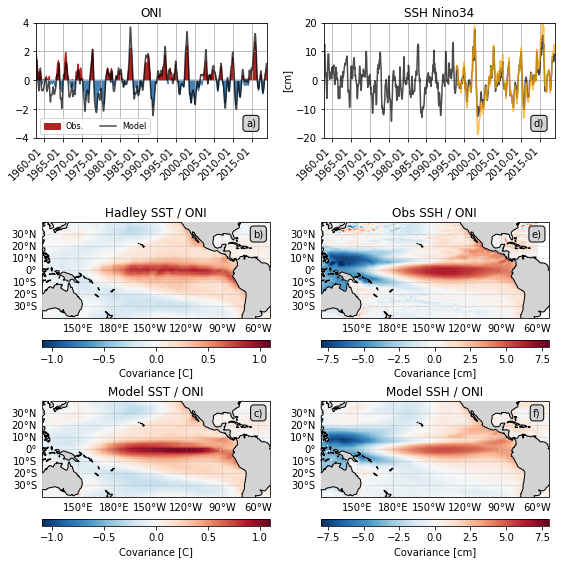
\includegraphics[scale=0.6]{figs/fig1.png}
	\caption{Observed and simulated ONI indexes (a). Covariance between the ONI index and the Hadley (b) and simulated SST anomalies (c). Observed and simulated sea-level anomalies averaged over the Nino34 region (d). Covariances between the ONI index and the observed (e) and simulated (f) sea-level anomalies.}
	\label{fig:nemo-had-sst}
\end{figure}

Modelled ENSO SST  pattern closely resembles the observed one. This pattern is characterized by warm SST anomalies (1°C) centred in the central and eastern equatorial Pacific  flanked by the traditional horseshoe cooling pattern in the western Pacific extending towards the subtropical north and south Pacific. This SST seesaw in the equatorial region is further accompanied by a shoaling of the thermocline in the west and a deepening in the east (not shown).

In addition to SST, satellite-derived sea-level anomalies have been compared with the simulated ones. First, the simulated sea-level anomalies averaged over the Nino34 region compare well with the observed ones (Fig \ref{fig:nemo-had-sst}d), with a correlation coefficient of 0.94. In addition, the spatial patterns associated with ENSO variability are very similar for both the observations and the model (Fig \ref{fig:nemo-had-sst}e, Fig \ref{fig:nemo-had-sst}f). Sea-level anomalies are negative in the western Pacific and positive in the central and eastern Pacific. These anomalies are consistent with thermocline vertical displacements, which shoal in the west and deepends in the east (\warn{REF}).

Covariance maps between the surface chlorophyll and the monthly ONI index are shown in Fig \ref{fig:nemo-sat-chl}. The observations (upper panel) and the model (lower panel) show very similar covariance patterns: El Niño induces a decrease in chlorophyll concentration along the equator east of 150°E, consistent with a weaker equatorial upwelling induced by the equatorial trade winds reduction. However, the model overestimates the chlorophyll response to ENSO variability compared with observational based estimates. Note that the covariance for the simulated chlorophyll has also been computed over the entire simulated period (1958-2018), with no significant changes in the resulting pattern (not shown).

\begin{figure}
	\centering
	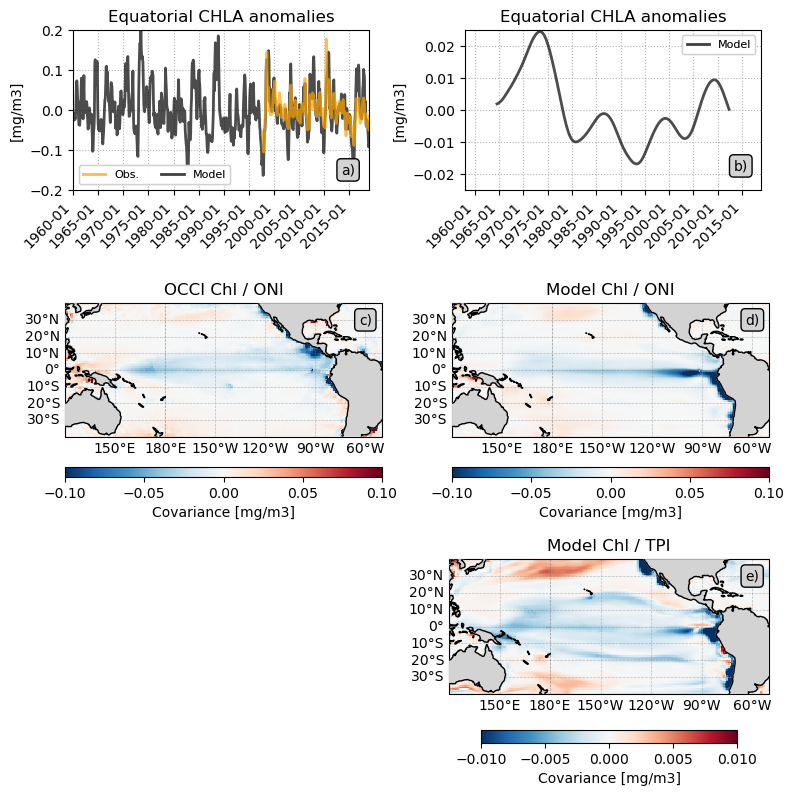
\includegraphics[scale=0.4]{figs/fig2.png}
	\caption{Simulated (black) and observed (yellow) equatorial chlorophyll anomalies (a). Filtered anomalies are shown for the model in panel (b). Covariance between the observed and simulated chlorophyll anomalies with the ONI (c, d) and filtered TPI (e) index.}
	\label{fig:nemo-sat-chl}
\end{figure}

% !TeX root = ../article-enso.tex

\subsection{Marine ecosystem model}
\label{sec:apecosm}

We use the Apex Predators Ecosystem Model (APECOSM, \citealp{mauryModelingEnvironmentalEffects2007, mauryOverviewAPECOSMSpatialized2010}) to simulate the energy transfer through marine ecosystems. 
APECOSM is a eulerian ecosystem model that represents the three-dimensional dynamics of size-structured pelagic populations and communities mechanistically. It integrates individual, population and community levels and includes the effects of life-history diversity with a trait-based approach \citep{mauryIndividualsPopulationsCommunities2013}. In APECOSM, energy uptake and utilization for individual growth, development, reproduction, somatic and maturity maintenance are modeled according to the Dynamic Energy Budget (DEB) theory \citep{koojmanDynamicEnergyBudget2010}. The DEB theory is a comprehensive mechanistic theory of metabolism. It has been extensively tested empirically. In APECOSM, it allows the dynamics of the main components of metabolism and life history and their size, temperature and food dependence to be represented together. In addition to metabolism, APECOSMP considers important ecological processes such as opportunistic size-structured trophic interactions and competition for food, predatory, disease, ageing and starvation mortality, key physiological aspects such as vision and respiration, as well as essential processes such as three-dimensional passive transport by marine currents and active habitat-based movements \citep{faugerasAdvectiondiffusionreactionSizestructuredFish2005}, schooling and swarming (see \citealp{mauryModelingEnvironmentalEffects2007, mauryIndividualsPopulationsCommunities2013, mauryCanSchoolingRegulate2017} for a detailed description of the model). 

As discussed in \cite{mauryIndividualsPopulationsCommunities2013}, size-based predation implies that predation rates are controlled by the ratio of sizes
between prey and predators (all organisms can be potentially predators and
preys at the same time, depending on their relative size, cf. equation D1 of \cite{mauryIndividualsPopulationsCommunities2013} for the detailed equation of the selectivity curve). Opportunistic predation implies that preys
of a given weight are eaten in proportion to their selected
available biomass relatively to the biomass of all possible preys
available.

All the metabolic rates are temperature-dependent and corrected by an Arrhenius factor \citep{mauryModelingEnvironmentalEffects2007, mauryIndividualsPopulationsCommunities2013}. While it can be prescribed in the model configuration, no preferred temperature range has been used in this study. Therefore, while temperature influences metabolism and swimming speed, its horizontal gradient does not influence the direction and magnitude of horizontal active swimming.

In APECOSM, the dynamics of communities is determined by integrating the core state equation below:

\begin{equation}
\partial_t \varepsilon = \underbrace{- \partial_w(\gamma \varepsilon) + \frac{\gamma}{w}\varepsilon}_{Growth} 
\underbrace{- M \varepsilon \vphantom{\frac{\gamma}{w}\varepsilon}}_{Mortalities}
\underbrace{-\overrightarrow{\nabla}.(\overrightarrow{V} \varepsilon) \vphantom{\frac{\gamma}{w}\varepsilon}}_{3D Adv} 
\underbrace{+ \overrightarrow{\nabla} . (D \overrightarrow{\nabla} \varepsilon) \vphantom{\frac{\gamma}{w}\varepsilon}}_{3D Diff.}
\label{eq:apecosm_trend}
\end{equation}

where $\varepsilon$  is the organisms' biomass density in the community, $w$ their individual weight, $\gamma$ is the growth rate, $M$ represents the different mortality rates (computed using equation 12 of \citealt{mauryIndividualsPopulationsCommunities2013}), $V$ and $D$ the sum of 3D passive and active velocities and diffusivity coefficients (computed following \citealt{faugerasAdvectiondiffusionreactionSizestructuredFish2005}). The growth contribution is made of an advection (i.e. the biomass transfer along the size-spectrum, left-hand side) and a source term (i.e. biomass creation, right-hand side). Reproduction is considered through a Dirichlet boundary condition that injects the reproductive outputs from all mature organisms in $w_0$.

In APECOSM, the energy ingested by organisms fuels individual metabolism according to the DEB theory. Ingestion is proportional to a functional Holing type II response function that depends on the size-dependent visibility of prey, their aggregation in schools and temperature. This functional response can be written in a simplified way as follows:

\begin{equation}
f_{c, w} = \dfrac
{P_{c, w}}
{
\dfrac
{C_{c, w} A(T)}
{h_c^{light} s_{c, w}(T)} + P_{c, w}
}
\label{eq:repfonct}
\end{equation}

with $P_{c,w}$ the prey biomass that is available to predator of community $c$ (see \citealt{mauryIndividualsPopulationsCommunities2013} for details) and size $w$, $C_{c,w}$ the half-saturation constant, $A(T)$ the
Arrhenius response of metabolism to temperature $T$, $h_c^{light}$
the response of vision to
ambient light and $s_{c,w}$ the predator speed.

In the APECOSM model, oxygen concentration only modifies the horizontal and vertical habitat of the different communities and size-classes and do not modify, in its current state, the  biological parameters or the physiological rates. Considering the region of interest of the given study, this limitation has barely no consequence. Which would not be the case if analysing outputs within an Oxygen Minimum Zone (OMZ). 

% \begin{displaymath}
% p_{c, u} = \sum_{k=1}^{N_{com}} \left[\int_{v=w_{egg}}^{w_{max}} P^{sch}_{k, v}\ s_{u, v}\ \xi_{k, v}\ dv\right] + \sum_{p=1}^{N_{ltl}} \left[ P^{sch}_{p}\ s_{u, p}\ \xi_{p}\right]
% \end{displaymath}

% \begin{displaymath}
% C_{c, w} = \frac{C_{REF}}{T_{ahr}\times h_c^{light}\times h_c^{tlim}\times W_{w}^{\chi}}
% \end{displaymath}

The APECOSM simulation used in this study is forced by three-dimensional temperature, horizontal current velocities, dissolved oxygen concentration, diatoms, mesozooplankton, microzooplankton and big particulate organic matter carbon concentrations \citep{aumontPISCESv2OceanBiogeochemical2015}, photosynthetically active radiation (PAR) and dynamic layer thickness outputs from the NEMO-PISCES simulation (section \ref{sec:nemo}). Nutrients concentrations simulated by NEMO/PISCES are not used as a forcing to Apecosm.

The APECOSM simulation runs with a daily time step for the biological processes, which is decomposed into a day/night cycle, the duration of which  depends on latitude and day of the year \citep{forsytheModelComparisonDaylength1995}. A sub time-stepping ($dt =0.8h$) is used for horizontal advection and diffusion to ensure numerical stability.

The depth dimension is explicit, i.e. each biological variable (mortality, functional response) is computed in 3 dimensions (depth, latitude, longitude). The vertical distribution is thus determined from habitat functions that depend on the choice of the communities. In this study, three interactive communities are simulated:
\begin{itemize}
\item{The epipelagic community, which includes the organisms that are feeding during the day near the surface such as yellowfin or skipjack tunas for example. Its vertical distribution is influenced by light and visible food during daytime as well as temperature and oxygen during both day and night, while its functional response is influenced by light and temperature.}
\item{The migratory mesopelagic community, which feeds in the surface layer at night and migrates to deeper waters during the day. Its vertical distribution is influenced by light and visible food during the night.}
\item{The resident mesopelagic community, which remains at depth during both night and day. Its vertical distribution is influenced by light and visible food during the day.}
\end{itemize}

To ensure that the size-spectrum is fully unfolded and a pseudo-steady state is achieved, the model was integrated successively over three 1958-2018 cycles. It was first initialized with an arbitrary small biomass value in each size-class and community and integrated from 1958 to 2018 (61 years). Then, the end of this first integration phase was used to run another cycle, which in turn was used to initialize the simulation analyzed in this study.

For each community, equation \ref{eq:apecosm_trend} is integrated over 100 logarithmically distributed size classes, ranging from $0.123cm$ to $196cm$. Since saving the outputs in 3D for the 3 communities and 100 size-classes is very costly, mortality rate, growth rate and functional response for each community and size are vertically averaged as follows:

\begin{equation}
F(y,x,c,w) = \frac{\sum_{z=0}^{H} F(z, y, x, c, w) B(z, y, x, c, w)}{\sum_{z=0}^{H}B(z, y, x, c, w	)}
\end{equation}

with $x$ the longitude, $y$ the latitude, $z$ the depth, $c$ the community, $w$ the size-class, $F$ the variable to consider (functional response, mortality rate, growth rate) and $B$ the 3D biomass (in $J.m^{-3}$).

In the remainder of the paper, the focus is solely put on the response of the epipelagic community; its near-surface location makes it more sensitive to ENSO variability \citep{lemezoNaturalVariabilityMarine2016}, it corresponds to organisms such as skipjack and yellowfin that are targeted by the industrial purse seine fleet, it accounts for the majority of tuna catches in the region, and have been reported to respond markedly to ENSO \citep{lehodeyNinoSouthernOscillation1997}.


%\section{Data and method}
%
%In the present section, the different observation-based datasets used in this study to validate the numerical models are presented. 
%
%%and statistical tools used in this study are presented.
%
%
%
%\subsection{Sea-level anomalies}
%\label{sec:ssh}
%
%Observation-based sea-level anomalies are obtained from the reprocessed Global Ocean Gridded L4 Sea-Surface Heights\footnote{\url{https://doi.org/10.48670/moi-00148}} data, provided by the Copernicus Climate Service as monthly values on a regular $0.25 \times 0.25$ grid from 1993-01 to 2020-12. This product was built by the DUACS multimission altimeter data processing system, which processes data from all altimeter missions: Jason-3, Sentinel-3A, HY-2A, Saral/AltiKa, Cryosat-2, Jason-2, Jason-1, T/P, ENVISAT, GFO, ERS1/2. Using along-track altimeter data, gridded sea-level anomalies are extracted by using an Optimal Interpolation off all the flying satellites. 
%
%%For our study, a monthly sea-level climatology was computed from 1993 to 2018 and used to extract monthly sea-level anomalies, which have been detrended.
%
%\subsection{Chlorophyll}
%\label{sec:chl}
%
%Chlorophyll observation-based estimates are extracted from the monthly OceanColour-CCI V5 CHL-a dataset\footnote{\url{http://dx.doi.org/10.5285/1dbe7a109c0244aaad713e078fd3059a}} \citep{sathyendranathOceanColourTimeSeries2019} over the 1997-09/2018-12 period. For our purpose, the high resolution dataset (4 km) has been regridded on a regular $1\times 1$ grid by computing weighted chlorophyll averages over $24\times24$ boxes, with the weights being provided by the cosine of latitude. When more than $1/3$ of the data used in the averaging is missing, the regridded cell is masked. 
%
%%The monthly climatology has then been computed over the 1998-2008 period and used to extract monthly anomalies, which have then been detrended.
%
%\subsection{Fish biomass estimates}
%\label{sec:fish}
%
%Fish biomass estimates are extracted from the IRD Level 2 global monthly catch of tuna, tuna-like and shark species dataset\footnote{\url{https://doi.org/10.5281/zenodo.1164128}} \citep{taconetGlobalMonthlyCatch2018}. First, the purse-seine captures of skipjack and yellowfin tunas have been extracted from the raw input file. Then, non-monthly observations (i.e. when the difference between the end and start dates exceed 31 days) have been discarded, as well as those which are unlocalized. Finally, the remaining observations have been regridded into on a regular $1 \times 1$ grid using the overlapping area between the observation polygon and the destination cell. The final product is a $3D$ array of dimensions (time and space) that extends from 1959 to 2016. However, due to the early poor data coverage, this dataset was used from 1985 onward.
%
%%\subsection{Covariance analysis}
%%\label{sec:cov}
%%
%%In order to assess the spatial signature of ENSO variability on physical, biogeochemical and biological variables, covariance analysis is used. For each grid cell, the monthly climatology of the analysed fields is removed, and the resulting monthly anomalies are detrended. Finally, the covariance between the detrended anomalies and the ONI index is computed. The resulting map can be interpreted as the monthly anomalies associated with an ONI value of 1.
%%%Correlations are computed in the same way. 
%%%Their significance has been inferred using a Student t-test, in which the effective number of degrees of freedom has been corrected based on the 1-lag autocorrelation of the 2 two time-series \citep{brethertonEffectiveNumberSpatial1999}.
\section{Response of the epipelagic community to extreme El Niño events}

This section describes the simulated response of the epipelagic community to ENSO as a function of organisms' size and analyses the underlying mechanisms. Here, we focus on  the marine ecosystem response to the three strongest El Niño events in the historical record, namely those of 1982/83, 1997/98 and 2015/16 \citep{santosoDefiningCharacteristicsENSO2017}. During these events, the central and eastern Pacific has warmed by more than 2°C (Fig\ref{fig:nemo-had-sst}a), displacing the warm waters and associated atmospheric convection from the western to the central Pacific. The atmospheric signature of these El Niño had dramatic climatic consequences, including droughts and wildfires, in countries bordering the western Pacific, but also torrential rains and flooding along the south American coast \citep{caiClimateImpactsNino2020}. Their oceanic signature also tremendously impacted marine ecosystems and biodiversity, leading to major disruption of marine life and seabird populations \citep{valleImpact198219831987}, promoting large-scale marine heatwaves \citep{holbrookKeepingPaceMarine2020} and coral bleaching \citep{claarGlobalPatternsImpacts2018}.  The response of the ocean during each of these three extreme events has been extensively described and analyzed in terms of physics  (e.g. \citealp{philanderChapter33Simulation1985, lengaigneOceanResponseMarch2002, puyModulationEquatorialPacific2019}), biogeochemistry (e.g. \citealp{barberBiologicalConsequencesNino1983, chavezBiologicalChemicalResponse1999, strammaObservedNinoConditions2016}) and marine ecosystems \citep{glynnNINOSOUTHERNOSCILLATION198219831988, glynnCoralBleachingMortality2001, eakin20142017Globalscale2019} 

In order to isolate the generic response of epipelagic communities to extreme El Nino events, independent of the intrinsic characteristics of each event, we perform a composite analysis of these three extreme events, averaging monthly anomalies of temperature, ocean velocity, low-trophic level concentrations (LTL, i.e. phyto and zooplankton, particulate organanic matter) and epipelagic commnunity biomass over the periods 1982-1984, 1997-1999 and 2015-2017. These extreme El Niño events are also followed by La Niña conditions in the following year (more intense in the case of the 1997/98 event), which also allows for a discussion epipelagic community response mechanisms to La Niña events. Although the temporal evolution and amplitude of the processes discussed below vary slightly between events, the relative importance of the processes discussed in our composite analysis remains the same when these three extreme events are analyzed individually (not shown). 

\subsection{Modeled upper-ocean response: from physics to ecosystems}

Because these are major environmental drivers of the epipelagic community biomass variability, we first describe in Figure \ref{fig:hov_nemo_ape}a-c the temporal evolution of monthly equatorial anomalies of the upper ocean temperature, chlorophyll concentrations and zonal currents during and after extreme El Niño events, in the form of equatorial time-longitude diagrams, whose time of origin is the January month before the onset of the El Nino event. The warming signal associated with El Niño begins in the central equatorial Pacific in early spring, spreads rapidly to the eastern Pacific, intensify during the summer and fall, peaks at the end of the calendar year, and finally rapidly declines and transitions to La Niña conditions the following spring (month 16, Fig.\ref{fig:hov_nemo_ape}a). The development phase of El Niño is also characterized by strong  eastward surface currents anomalies in the western and central Pacific (Figure \ref{fig:hov_nemo_ape}c) induced by anomalous westerly winds, promoting warming of the the central Pacific and eastward movement of the warm-pool to the eastern equatorial Pacific. These current anomalies reverse at the peak of El Niño and during La Niña. The simulated plankton concentration anomalies largely mirror those of temperature, with a strong decline during El Niño and an increased bloom during La Niña (Figure \ref{fig:hov_nemo_ape}.b). 


\begin{figure}[h!tp]
	\centering
	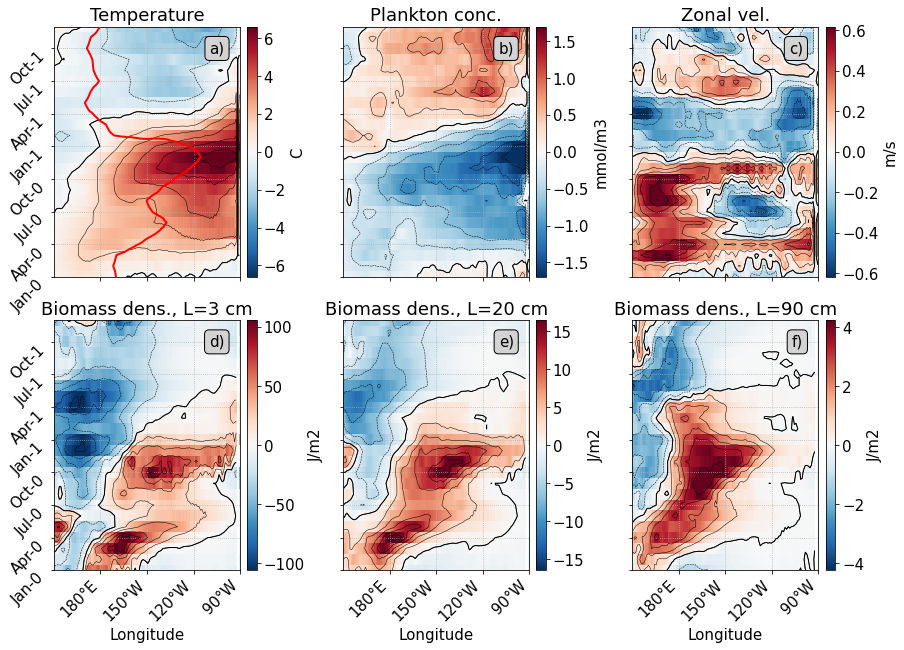
\includegraphics[scale=0.4]{plot_all_hovmoller_phys_oope.png}	
	\caption{Hovmoller diagrams of equatorial temperature (a), low-trophic level concentrations (b), zonal velocity (c) and fish biomass anomalies (3cm, 20cm and 90 cm in d, e, f, respectively).}	
	\label{fig:hov_nemo_ape}
\end{figure}

A similar analysis is then performed for epipelagic biomass for the three size classes we selected (Fig\ref{fig:hov_nemo_ape}d, Fig\ref{fig:hov_nemo_ape}e and Fig\ref{fig:hov_nemo_ape}f). Their responses to El Niño share some common features: positive biomass anomalies appear near the dateline at the beginning of the the calendar year and propagate eastward toward the central Pacific until late spring (May/June). This positive biomass anomalies in the central Pacific re-intensify in fall and quickly disappear in winter. They are also accompanied by a decrease in biomass in the western Pacific from the summer of the El Niño year. These negative anomalies persist after the El Niño peak and during the subsequent La Niña event but remain largely confined to the western Pacific. However, there are significant differences in the behaviour of the three size classes, including a westward-shifting response size classes increase.

The analysis of the trend terms (equation \ref{eq:apecosm_trend}) allows us to identify the role of the processes responsible for the response of the epipelagic community to El Niño highlighted in Figure \ref{fig:hov_nemo_ape} by analysing the associated tendency terms (equation ??). The same hovmuller diagrams are made for the main trend terms (right members of \ref{eq:apecosm_trend}) and for their integral representing their contribution to the total biomass change. We also analyze various key parameters of the biological response to changing environmental conditions, namely growth rate ($\gamma$ in equation \ref{eq:apecosm_trend}), functional response and predation mortality rates ($M$ in equation \ref{eq:apecosm_trend}). Because the relative importance of these processes varies with the size classes, these analyses are discussed separately for each size class.

\subsection{Processes driving epipelagic upper-ocean response}

Figure \ref{fig:fig7} presents a synthesis of the respective contribution of biological (i.e. the combined action of growth and predation) and physical (i.e. the combined action of advection and diffusion) processes on the epipelagic biomass response to ENSO for three size classes. For the largest size class, physical processes (Fig \ref{fig:fig7}i) explain most of the biomass changes (Fig \ref{fig:fig7}g), with biological processes being an order of magnitude smaller (Fig \ref{fig:fig7}h). The increase in biomass in the central Pacific and decrease in the west is consistent with passive transport of large organisms by ocean currents from the western to the central Pacific. This advection is due to the strong eastward current anomalies simulated in the western and central Pacific during the onset and development phase of an extreme El Niño (up to 0.6m/s; see Fig\ref{fig:hov_nemo_ape}c). While the influence of passive horizontal transport by currents dominates active movements and is broadly similar for all size classes, the relative importance of biological processes increases as fish size decreases. The decrease in biomass in the western Pacific is indeed primarily the result of biological processes for intermediate and small size classes. In the central and eastern Pacific, the combined action of dynamical and biological processes explain biomass increase during El Niño (Fig \ref{fig:fig7}a-f) while these processes largely cancel each other when the equatorial Pacific reverses to La Niña conditions, resulting in small biomass changes in this region. There are two main reasons why the relative importance of biological processes decreases with increasing size. First, predation is size-based in APECOSM, resulting in high predation pressure on small organisms, which decreases with size since larger organisms have no predators in the model. The second important biological process that affects biomass is growth, which includes a flux term and a source term (see equation \ref{eq:apecosm_trend}) that are both temperature-dependent. The source term controls biomass production. It varies as ${\gamma}/{w}$, which scales linearly with $w^{-\frac{1}{3}}$ and thus decreases sharply with size.


\begin{figure}[h!tp]
	\centering
	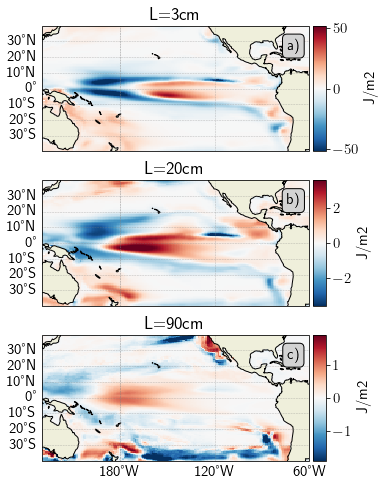
\includegraphics[scale=0.4]{figs/fig7.png}	
	\caption{Total (left), biologically (predation and growth, middle) and dynamically (right, advection and diffusion) induced changes in fish biomass for small (top), intermediate (middle) and large (bottom) sizes.}
	\label{fig:fig7}
\end{figure}

The influence of dynamical processes is simple. It results from the transport of biomass from the western to the central Pacific due to the strong eastward currents appearing during extreme El Niño conditions. It is experienced by all size organisms. The significant and sometimes dominant contribution of biological processes for small and medium size classes is, however, more difficult to understand intuitively as it results from the combined action of predation mortality and growth. Therefore, we further detail the respective contribution of predation and growth and their driving factors for small and medium size classes on Figures \ref{fig:fig8} and \ref{fig:fig9} respectively. For small size classes (3cm), the effects of predation mortality balance the effects of growth (Fig. \ref{fig:fig8}a and Fig. \ref{fig:fig8}.b), which results in a net effect of biological processes two to three times smaller than the effect of physical processes (Fig. \ref{fig:hov_nemo_ape}d). Growth leads to an increase  of biomass in the central Pacific (between dateline and 150\degree{}W) at the onset of El Niño, expanding eastward until its peak. These positive biomass anomalies then decrease slightly during the following La Niña conditions. This evolution can be related to the evolution of the modeled growth rate, which increases in the central and eastern Pacific during El Niño and decreases slightly during the following La Niña, matching closely the evolution of temperature. Since changes in growth rate are largely driven by temperature, the anomalous warming observed east of the dateline during El Niño increases the growth rate and thus the biomass of small size classes due to the source term associated to growth in equation (1). Conversely, the cooling observed during the subsequent La Niña conditions decreases the growth rate, dampening the El Niño-induced increase in biomass. In contrast to the central and eastern Pacific, the growth rate decreases in the cooling western Pacific from June of the El Niño year and this contributes to a decrease in biomass, which reverts during the following La Niña. Again, temperature changes have a major influence on growth rate and biomass of small size class organisms. Despite its importance in controlling growth and reproduction, Fig. \ref{fig:fig8}.e shows that the functional response is indeed not the main driver here, as its influence is two orders of magnitude smaller than the the temperature-driven biomass changes induced by growth. The functional response show negative anomalies that are consistent with the reduction of low-trophic level prey concentrations modulated by temperature, which controls the swimming speed of predators (attack rate of the Holling type 2 functional response), and the vertical distribution and swarming level of low trophic level prey, which control their availability to predators. As mentioned earlier, changes in biomass induced by predation largely mirror those induced by growth. They act to decrease biomass in the central and eastern Pacific and increase it in the western Pacific, closely following the biomass changes of intermediate size predators. Despite their opposite effect on biomass, the effects of growth dominate those of predation, explaining most of the decrease of small sized biomass in the western Pacific during El Niño and the subsequent La Niña and enhancing the biomass increase in the central Pacific induced by dynamical processes during El Niño.  

\begin{figure}[h!tp]
	\centering
	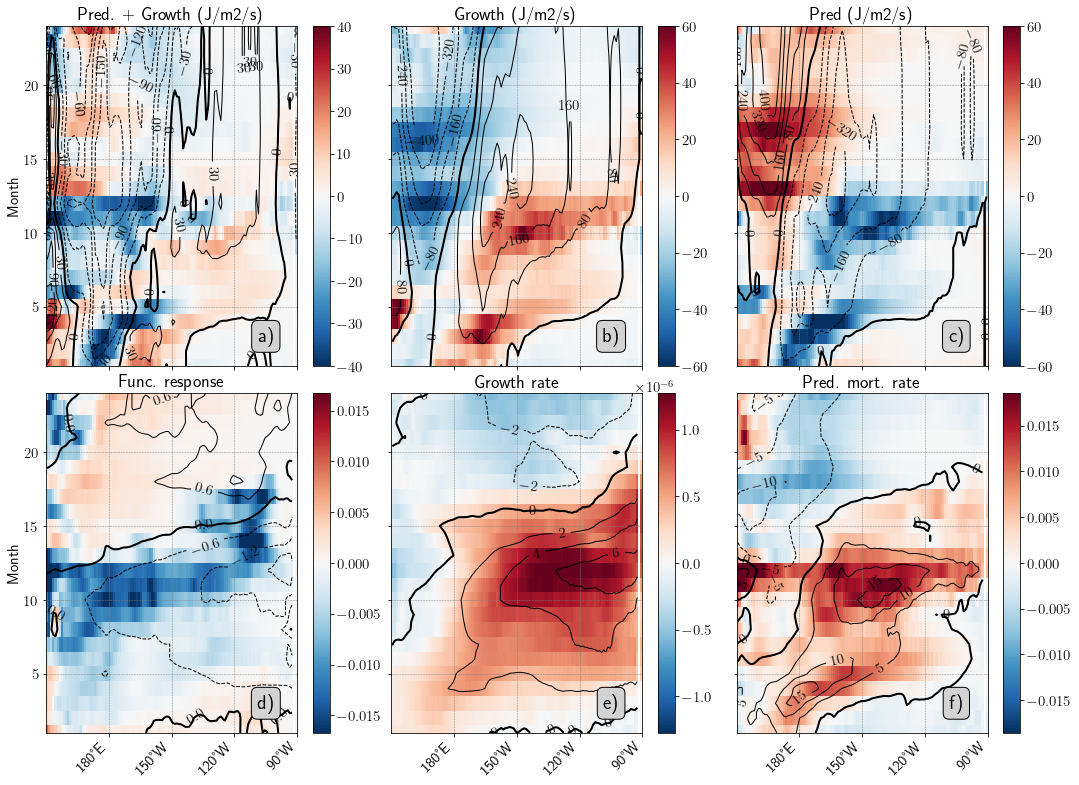
\includegraphics[scale=0.4]{figs/fig8.png}	
	\caption{Small sizes biological trends (colors) and time-integrated trends (contours) (a, b and c). Functional response (colors) and plankton (contours) anomalies (d). Growth rate (colors) and temperature (contours) anomalies (c). Predation mortality rate (colors) and intermediate biomass anomalies (f).}
	\label{fig:fig8}
\end{figure}

Biomass changes induced by growth and predation for intermediate size classes are similar to those simulated for small size classes: they are opposite and of the same order of magnitude but overall, the effects of growth dominate those from predation. Growth increases fish biomass in the central Pacific from the onset to the peak of El Niño, while it decreases the biomass in the western Pacific during the subsequent La Niña. However for intermediate size classes, the influence of temperature on fish physiology is not anymore the dominant factor of biomass changes from biological processes as it was for small organisms. As opposed to small size classes, growth rate changes reflect changes in the functional response, which increases in the central Pacific both because of warmer waters (increasing swimming speed that controls the attack rate parameter in the functional response) and increased food availability due to the increase of small organisms' biomass. These processes contribute to increasing the biomass of intermediate size organisms. In the western Pacific, the growth rate doesn't change much (Fig. \ref{fig:fig7}b). This is because the intermediate size organisms change their vertical distribution (from around 60m to around 30m, cf. Fig. \ref{fig:fig8}e) pushed by the shallowing of the thermocline and concentrate at the depth of their prey so that they do not experience neither substantial prey changes (Fig.\ref{fig:fig8}d) nor water cooling (Fig.\ref{fig:fig8}a). The source component of growth is therefore not changed but the advective flux along the weight axis (see equation \ref{eq:apecosm_trend}) decreases during La Niña (Fig. \ref{fig:fig7}a) because of the biomass decrease induced both by passive eastward advection by marine currents during El Niño and increased mortality rates (Fig. \ref{fig:fig7}d). However, predation acts to dampen the effects of growth, reducing biomass in the central Pacific because of increased predation by large size classes there and increasing biomass in the western Pacific during the subsequent La Niña because of reduced predation. The changes induced by the combination of both processes is dominated by growth however and resembles the one obtained for small sizes albeit a modest westward shift. As for small sizes, the biomass decrease in the western Pacific during El Niño and the subsequent La Niña is largely driven by a growth reduction, while dynamical processes dominate the biomass increase east of the dateline with a smaller contribution from growth.  The comparison of active and passive velocities suggests that passive movements (i.e. advection by the ocean currents) dominate, with ocean current anomalies greater than active velocity anomalies by a factor of $\approx\ 20$.

\begin{figure}[h!tp]
	\centering
	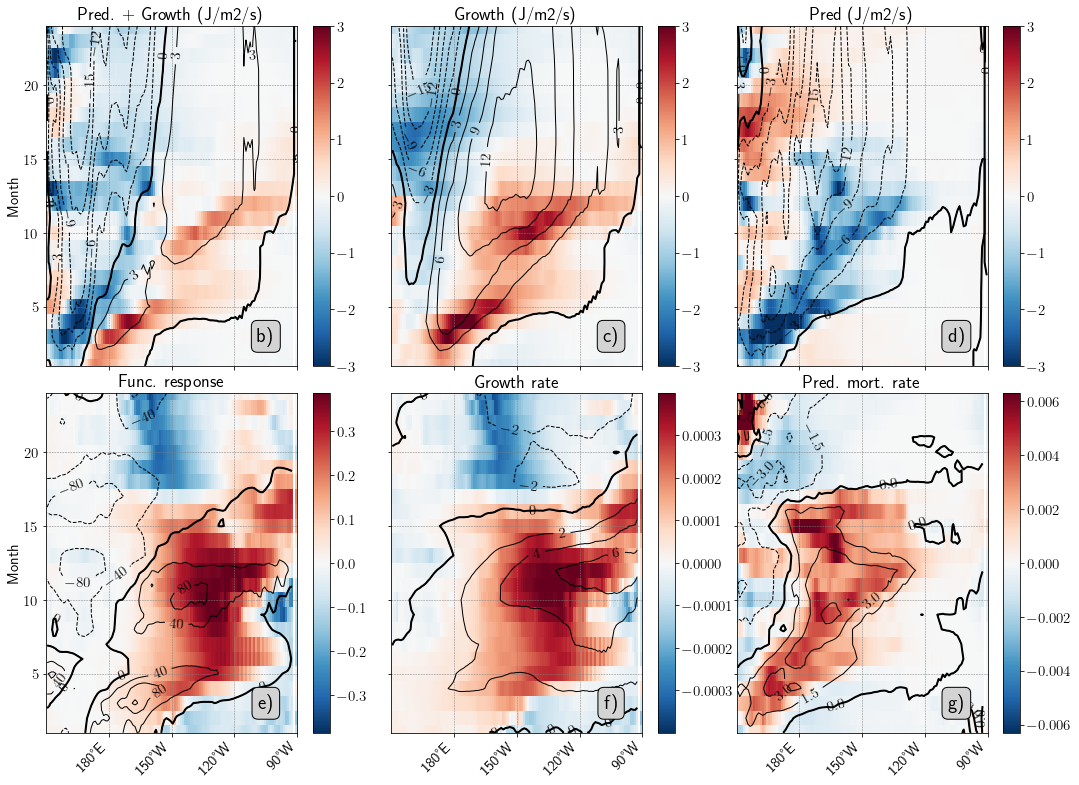
\includegraphics[scale=0.4]{figs/fig9.png}	
	\caption{Intermediate sizes trends (colors) and time-integrated trends (contours) for growth and predation (a and b). Growth rate (colors) and temperature (contours) anomalies (c). Predation mortality rate (colors) and large biomass anomalies (d). Functional response (colors) and small biomass (contours) anomalies (f).}	
	\label{fig:fig9}
\end{figure}

Changes in large fish biomass are dominated by advection/diffusion transport processes, while predation and growth have virtually no impact because their importance decreases structurally with size (see above). 

%ADD HERE A SMALL PARAGRAPH SUMMARIZING THE DOMINANT PROCESSES DRIVING BIOMASS SHIFT FOR ALL SIZE CLASSES.

\subsection{Subsurface response}

Figure \ref{fig:profiles} shows the mean equatorial profiles for temperature, zonal velocity, low-trophic level concentration and fish-biomass (contour lines) and the composites of OND El Nino anomalies. Mean temperature exhibits a deep thermocline in the western Pacific and a shallow one in the east, which flattens during El Nino, leading to a warming in the east and a cooling in the west. The structure of the Equatorial Undercurrent is clearly visible on the zonal velocity profile. It strongly weakens during El Nino, while strong positive (i.e. eastward) anomalies occur near the surface. Low-trophic level biomass is maximum in the top 50m of the eastern Pacific and decrease during El Nino, due to the flattening of the thermocline, which is associated with a decrease in nutrient supply.

Right columns of Fig \ref{fig:profiles} show the equatorial profiles of fish biomass density for the three size-classes under focus here. On average, biomass in the western Pacific reaches $100m$, while in the eastern Pacific, it remains very close to the surface $25m$. The western biomass for small sizes is maximal close to the surface near the dateline, while for intermediate and large sizes, the maximum occurs deeper, around $40m$ in the western Pacific (between 150 and 160\degree{}E)
During El Nino conditions, fish biomasses increase in the eastern Pacific (except very close to the surface) and a decrease in the west. However, the latter is not homogeneous on the vertical, since strong positive anomalies appear around 40m in the east for intermediate and large sizes. These are induced by a tightening of the vertical habitat, due to the shallowing of the thermocline.

\begin{figure}[h!tp]
	\centering
	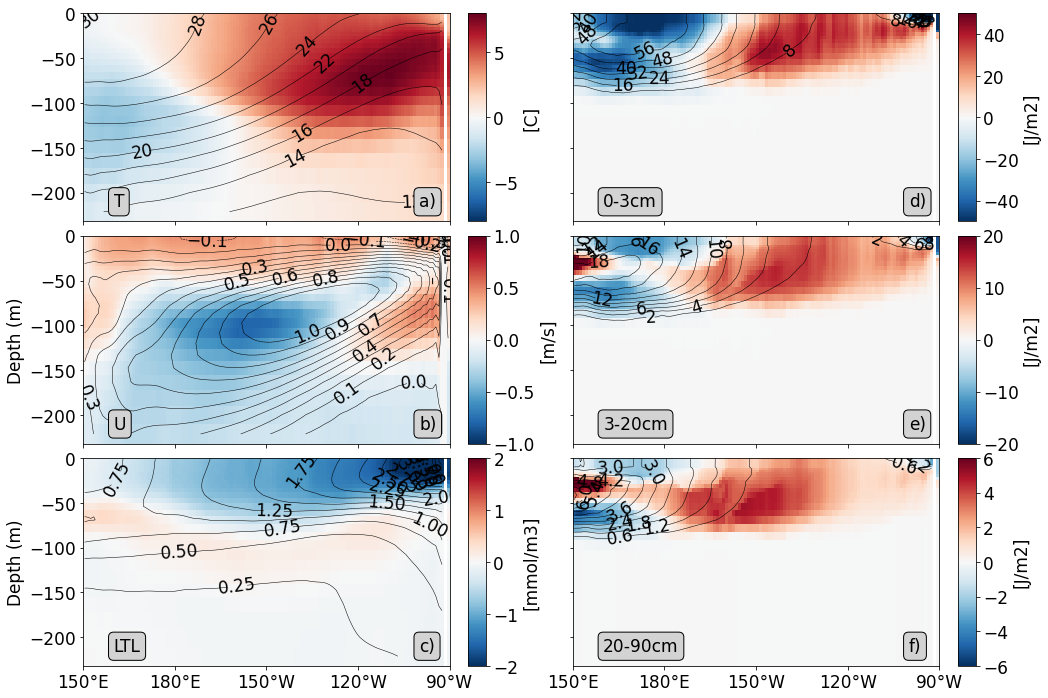
\includegraphics[scale=0.4]{figs/forage_mean_ond97.png}	
	\caption{Pacific equatorial profiles of temperature (a), zonal velocity (b), low-trophic concentration (c) and fish biomass (d for small, e for intermediate and f for large sizes). Mean are represented as black contour lines and El Nino anomalies are represented in colors.}	
	\label{fig:profiles}
\end{figure}

\subsection{Generalization}

Figure \ref{fig:mean_ond97_ape} shows that, in average, small epipelagic fish biomass is maximal around 5\degree{}N and 5\degree{}S (see the $2.0$ contour Fig \ref{fig:mean_ond97_ape}a), while smaller biomasses are found at the equator and in the eastern Pacific. During El Nino, anomalies calculated using our composite of the three extreme events indicate an equatorward and an eastward shift of biomass.
As size increases, the location of the equatorial biomass minimum in the central and eastern Pacific extends westward and poleward, while the positive anomalies associated with El Nino conditions follow the same pattern: for intermediate sizes (Fig\ref{fig:mean_ond97_ape}b), the positive anomalies reach 180\degree{}E, while for small sizes, the anomalies are located east of 150\degree{}W. 

\begin{figure}[h!tp]
	\centering
	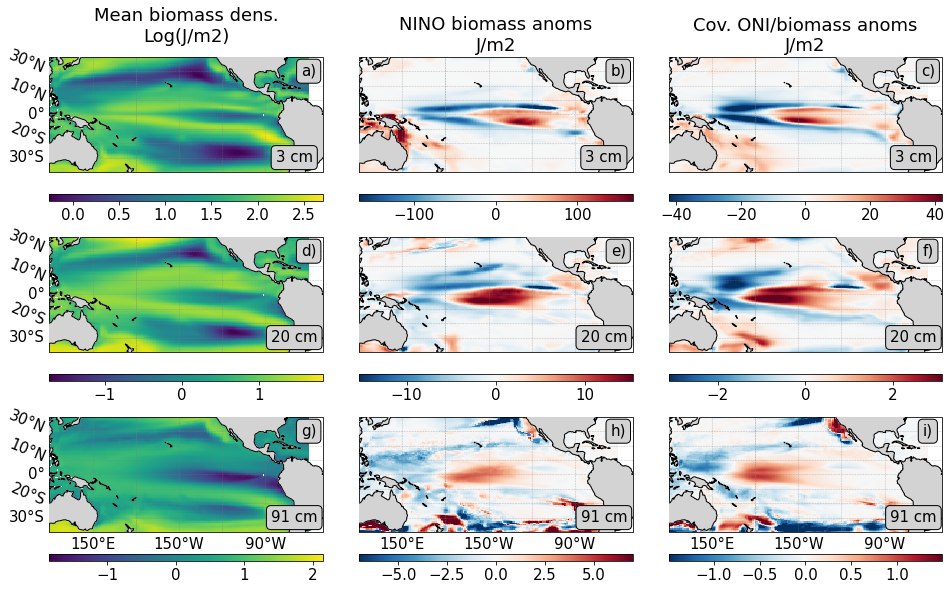
\includegraphics[scale=0.4]{figs/map_mean_anom_OND_97.png}	
	\caption{OND-NINO anomalies (left column) and covariance of fish biomass anomalies with the ONI index (right column) for small (upper line), intermediate (middle line) and large sizes (lower line). Black contours show the contours of mean fish biomass density (log-scale).}	
	\label{fig:mean_ond97_ape}
\end{figure}

%The patterns of the functional response and growth rates are very different for small sizes (figures YYY.a and YYY.d). The former shows negative anomalies on the central Pacific during the onset of El Nino conditions, presumably due to the concomitant reduction of plankton concentration (figure YYY.b). Interestingly, no anomalies are found in the eastern basin, due to compensating effects of warming temperatures and reduced plankton concentrations. The growth rate shows a pattern that is very similar to the temperature anomalies (Fig. XXX.a), indicating the dominance of temperature on the growth rate. The mortality rate (Fig. YYY.g) shows a pattern that is consistent with the increased biomass of intermediate epipelagics (XXX.b), which predate on small ones.  Besides, growth rate anomalies superimpose well on the small biomass anomalies (black contours in Fig. YYY.d), hence suggesting that the increased biomass during the El Nino conditions is triggered by enhanced growth associated with warmer temperature, despite a dampening effect of increased mortality rates.
%For intermediate sizes, the functional response and the growth rate show very similar anomalies, hence suggesting that they both are driven by the same factors. Both show positive anomalies during the onset of El Nino between 200E and 250E, presumably induced by the temperature warming that favours both the growth and search rates. Then negative anomalies occur, which are westward shifted relative to the positive ones. These negative anomalies are likely induced by the cooling associated with the La Nina conditions reinforced by the reduced small fish biomass that appears near 200E, as shown in Fig. XXX.d. Mortality rates anomalies are consistent with the increase of large fish biomass (Fig. XXX.f). Comparing the different fields, we can suggest that the increased fish biomass that appears on the central Pacific in early 1997 is first dominated by advective processes, which returns a similar pattern (fig YYY.k). Then, during the El Nino peak, the increased biomass of intermediate fish is driven by both an increased growth rate and an increased functional response, which are induced by warmer temperatures and more food available (more small epipelagic fishes, Fig. XXX.d).

%\subsection{Generalisation}
%
%In order to see if ecosystem response to the 97 El Nino event is representative, the covariance between fish biomass anomalies and the ONI index have been computed, following the methodology described in section \ref{sec:cov}. The maps are presented in Fig\ref{fig:ape_cov}.
%
%\begin{figure}
%	\centering
%	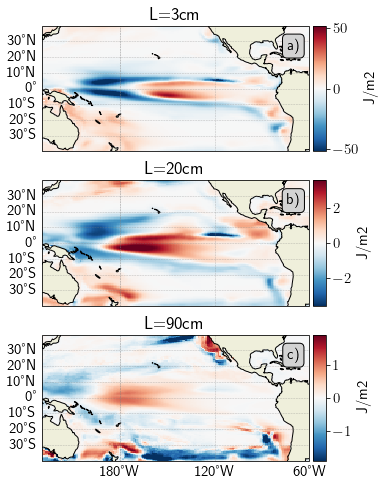
\includegraphics[scale=0.6]{figs/fig7.png}	
%	\caption{Covariance maps between the ONI index and the vertically integrated fish biomass anomalies for small (a), intermediate (b) and large (c) sizes.}	
%	\label{fig:ape_cov}
%\end{figure}
%
%The covariance patterns are very similar to the biomass anomalies depicted in Fig\ref{fig:mean_ond97_ape}, therefore suggesting that the mechanisms described in the above  apply to the general case. However, we note that the covariance patterns are westward shifted compared to the fish biomass anomalies. 
%
%This westward shift might be explained by the fact that when performing covariance anomalies, different El Nino events (Easter Pacific El Nino, Central Pacific El Nino) and La Nina events are considered, which ultimately impacts the global view of fish biomass response to ENSO variability.


%In this section, the interannual response of epipelagics to ENSO variability is investigated using covariance analysis. The left panels of Figure 3. show the yearly mean vertically integrated fish biomass over the entire simulation for the three different size classes. For small sizes (Figure 3a), the fish biomass is concentrated at around 10° S and 10 ° N in the central Pacific and close to the equator in the western Pacific. High biomass concentration is also found east of 90° W, off the coasts of Chile. As size increases, the equatorial "blue spot" extends meridionnally and to the west. This pattern is mostly driven by the active and passive advection of fishes in the Apecosm model (REF). Without advection, the biomass will be concentrated at the equator, where the plankton concentration is the maximum.
%
%Covariance maps between vertically integrated fish biomass and the winter ONI index are shown in the right panels of Figure 3. Small epipelagics show negative anomalies in the Western Equatorial Pacific and positive anomalies in the Central Equatorial Pacific. This pattern can be interpreted as an eastern displacement of the mean biomass in the Western Pacific. Similar dipolar patterns are also obtained for intermediate and large sizes, but the anomalies westward shifted as size increases. This can be interpreted, as for small sizes, by a westward shift of fish biomass during positive El Niño phases. The same results have been obtained when the covariance analysis is performed on monthly anomalies (not shown).


In order to insure that our composite of extreme El Nino events give a robust view of the response of fish biomass to ENSO, covariance maps are computed between the monthly ONI index and the detrended fish biomass anomalies over the 1958-2018 period (right column of Fig\ref{fig:mean_ond97_ape}). The El Nino composites and the covariance maps are very similar, despite anomalies slightly shifted westward and lower amplitudes for the covariance maps compared to the composites. These  differences are due to the fact that covariance analysis includes Central Pacific (i.e. Modoki) El Nino events (such as the 1986, 1991, 1994, 2002, 2004 and 2009 events) and La Nina events, whose signature is not opposite to Eastern Pacific events. Nevertheless, the very good agreement between the covariance maps and the El Nino composites suggests that our focus on the three major events gives a robust view of fish biomass response to ENSO.
% !TeX root = ../article-enso.tex

\section{Conclusion and discussion}
\label{sec:conclusion}

%Summary of our results:

\subsection{Conclusion}

% (1)
ENSO, the most energetic interannual climate mode on a  global scale, is known to strongly impact marine ecosystems through changes in habitat conditions (oxygen, temperature, light penetration), currents and food availability. In particular, tuna catch data point to a shift of epipelagic biomass from the equatorial western to the central Pacific in response to El Niño and an accumulation of the biomass in the extreme western equatorial Pacific in response to La Niña. These indirect and heterogeneous data, which do not solely reflect changes in fish populations, do not allow to address the mechanisms responsible for these changes. Here, we use a simulation from a mechanistic ecosystem model that captures the zonal shift of the epipelagic community in response to ENSO similar to the response of tuna catches and allows, through the analysis of the tendency terms of biomass changes, to unravel underlying mechanisms.

% (2)
Despite a relatively similar modeled response of epipelagic communities to El Niño among different size classes, characterized by a decrease in biomass in the western Pacific and an increase in the central Pacific, our analyses reveal that the processes responsible for these changes vary considerably by size. For large organisms,  eastward passive transport by El Niño-related eastward surface currents anomalies is largely responsible for the movement of organisms from the western to the central Pacific and dominates the effects of growth and predation, which are structurally weaker for large organisms. For intermediate-sized organisms, while the increase in biomass in the central Pacific is also largely explained by eastward advection by zonal currents anomalies, the decrease in biomass in the western Pacific is explained initially by increased predation by large organisms, and then by reduced growth due to a decrease in the functional response related to both colder waters and decreased food availability. For small organisms, changes in growth rate  induced by the influence of temperature on fish physiology are an important process, reinforcing the increase in biomass induced by passive horizontal transport in the eastern Pacific and the decrease in biomass induced by increased predation by intermediate organisms near the dateline.

% (3) 
%The model simulates important effects of ENSO on the vertical distribution of organisms, with a shallower and more pinched vertical distribution in the west and deeper and less pinched in the central and eastern tropical Pacific during El Nino events.

\subsection{Discussion}
%Discussion:

% (1) 
Previous studies (e.g. \citealp{lehodeyNinoSouthernOscillation1997, lehodeyPelagicEcosystemTropical2001}) have attributed the eastward biomass shift of skipjack tuna during El Niño to active swimming to track the eastward migration of favorable warm waters. Here we show that such a biomass shift can be realistically simulated without the need to specify temperature preferences that would lead to active movements of the tuna towards the most favorable waters. Passive horizontal transport by ENSO-related currents is indeed sufficient in our simulations to explain the eastward movement of tunas. Our study highlights that it is therefore essential that marine ecosystem models account for the dynamical role of ocean currents in shaping the spatial distribution of marine communities and their response to climate variability.

%(2) 
Our analysis demonstrates the added value of using a mechanistic ecosystem model to disentangle the role of the different processes controlling biomass changes and understand their interactions. The analysis of biomass tendency terms is particularly powerful to isolate the effects of dynamical processes (passive transport by currents) from those of biological processes (growth, reproduction and predation in particular), and understand how these different processes change with environmental conditions and with organism size. Thus, the mechanistic foundations of the APECOSM model, which is based on the DEB theory, are particularly well suited to an in-depth analysis of the processes involved.

%(3) 
While La Niña has long been largely considered a mirror image of El Niño, the study of asymmetries between these two phases of ENSO has recently become an important research topic (e.g., \citealt{anENSOIrregularityAsymmetry2020}). This interest is firstly driven by an amplitude asymmetry, where the most intense El Niño events reach much larger amplitudes than the most intense La Niña events, but also by a spatial structure asymmetry, where La Niña SST anomalies are shifted westward and have a wider meridional extent compared to that of El Niño (e.g. \citealt{takahashiENSORegimesReinterpreting2011}). In this study, we focused primarily on the ecosystem response to extreme El Niño events because of their dramatic ecological and socioeconomic consequences. However, our analyses indicate that the epipelagic response to La Niña events that typically follows extreme El Niño is far from a perfect mirror image of El Niño (Fig. 4d-f), with the increase in biomass associated with extreme El Niño located in the central/eastern equatorial Pacific, while the decrease in biomass associated with the following La Niña remains confined to the western Pacific. These asymmetries associated with this ecosystem response also appear to be considerably larger than those associated with the physical response (Figure 4a) or the chlorophyll response (Figure 4c). A more refined assessment of the asymmetries in the response of marine ecosystems to ENSO and their associated driving processes is outside the scope of this study but deserves to be explored in detail in the future.

% (4) 
Although the historical simulation from our ecosystem model compares favorably with observations, it nevertheless has a number of limitations that deserve discussion. First, the model configuration used here corresponds to the level of generality that has been used in FishMIP to date. It simulates a single generic community for epipelagic organisms and two mesopelagic communities. We thus did not implement any temperature limitation to be as generic as possible and do not take into account the specifics of tuna physiology. Since these specifics are likely to affect the results, configuring APECOSM to specifically represent tuna species would help to refine our findings for particular species. We were also surprised to find that the role of active movements is negligible compared to passive movements, even for large organisms. Since this result may suggest an underestimation of active transport in our simulation, it is important to estimate more precisely the value of the movement parameters used from tagging data for example, and to study the sensitivity of our results to the value of this parameter.

% (5) 
Among the future developments envisioned, our modelling framework allows for sensitivity experiments where the interannual variations in key environmental factors (temperature, currents, food) can be artificially frozen to separate their relative influence on the food web dynamics. We also plan to examine the ENSO-related response of mesopelagic communities that are also explicitely simulated by our model. Finally, we plan to extend our analysis to other regions subject to significant climate variations, such as the Indian Ocean, which is home to the Indian Ocean Dipole (IOD), and to the analysis of climate change effects at the global scale. While the latter has been the focus of several recent studies (e.g. \citealp{lotzeGlobalEnsembleProjections2019, tittensorNextgenerationEnsembleProjections2021}), and the factors responsible for the strongest climate impacts discussed (e.g. \citealp{heneghanDisentanglingDiverseResponses2021}), a finer mechanistic analysis of the bio-ecological processes that climate change would bring into play in global marine ecosystems has not yet been conducted.

% Conclusion:
Reliable estimations of the magnitude of the impact of climate change on marine ecosystems and associated ecosystem services requires reliable numerical projections. Significant progress has been made in terms of modeling marine ecosystems and using them to project the impact of possible future climate change and construct relevant ensemble analyses (e.g. \citealp{lotzeGlobalEnsembleProjections2019, tittensorNextgenerationEnsembleProjections2021}). These analyses have notably contributed to the work of the IPCC \citep{portnerIPCCSpecialReport2019, portnerClimateChange20222022} and IPBES \citep{brondizioGlobalAssessmentReport2019} and it is important that the scientific community maintains this effort. However, the ability of the models used in these projections to reproduce the effects of past climate variability on ecosystems has not been thoroughly assessed yet, in particular due to the lack of relevant synoptic observations of high trophic levels. Yet, such an assessment is necessary and should be conducted to increase our confidence in these projections.

Finally, the magnitude of the expected climate change is such that marine ecosystems will operate in states without known analogues in the past. Mechanistic studies based on the fundamental principles governing the effects of past climate variability on marine ecosystems are very important in this regard. They help us to better understand the mechanisms that will be at play in those future no-analogue situations, when projections based on statistical analysis may become invalid. This can only increase our confidence in the future response projected by integrated ecosystem models to climate change, and allow us to better understand their diversity.
%\section{Discussions}

In the present paper, we analysed the response of fish biomass to changes in the physical and biogeochemical ocean in response to ENSO variability. The Apecosm model was forced by the outputs of the NEMO/Pisces physical and biogeochemical model, with no retroaction of the former on the latter. One question that arises is whether the response of fish biomass and ocean biogeochemistry to ENSO variability would be the same in a two-way coupled simulation. 	Such coupling, which has already been used in \cite{aumontEvaluatingPotentialImpacts2018} to analyse the impacts of the diurnal vertical migration on ocean biogeochemistry, could be used to determine whether the inclusion of fish biomass modifies the response of ocean biogeochemistry to ENSO. And whether the coupling attenuates or strengthens the response of fish biomass. Improve the text.
 
The study relies on a global simulation at a relatively coarse horizontal resolution (around 1°), which is insufficient to explicitly represents the mesoscale features of the California Current System \citep{capetMesoscaleSubmesoscaleTransition2008} and of the Peru-Chile current system \citep{colasHeatBalanceEddies2012}. This may lead to a misrepresentation of temperature and biogeochemical variables in the upwelling systems, which will ultimately propagates to the higher trophic levels. Guiet et al. (in prep) have used Apecosm on a regional configuration of the California Current Ecosystem. They show that small sizes emerge from the coast, where they are trapped in mesoscale features where plankton biomass is abundant, and are advected westward while they grow.

In this study, the transient response of marine ecosystems has been investigated from covariance analysis using a single El Nino index. This methodology assumes that ENSO variability is linear, i.e. that positive ENSO phases (El Nino) are opposite to negative ENSO phases (La Nina), which is not the case \citep{larkinENSOWarmNino2002}. Furthermore, no distinction has been made between the Eastern Pacific Nino (EPN) and the Central Pacific Nino (CPN) events, which have different physical and biogeochemical signatures and causes. For instance, \cite{gierachBiologicalResponse19972012} have shown, using satellite observations and adjoint passive tracer simulations, that EPN causes a reduction chlorophyll-a in the Eastern Pacific, mainly due to weaker trade winds, reduced upwelling and vertical mixing, while CPN reduces chlorophyll-a in the Central Pacific, mainly through a stronger eastward advection of nutrient-depleted waters from the Western Pacific. These different type of El Nino events may therefore have different impacts on fish biomass.

In the present study, changes in fish biomass in relation with ENSO variability are potentially driven by changes in temperature, oxygen or plankton concentration. In order to distinguish these different effects, sensitivity simulations can be run, for instance by using a temperature climatology instead of an interannual one. 

• Coupling NEMO-Pisces and impacts?  % done
• Regional simulations to better represents physical processes? %done
• Focus species (tuna), more suited for tropical pacific
• ENSO impacts in the other regions (cf. Racault)  
• Separation of CP/EP Ninos  % done
• Different communitities
• Sensitivity experiments (climPlk, climTemp)
• Impacts of other modes of variabilities (PDO, NAO, AR).

\warn{\cite{racaultImpactNinoVariability2017} for impact on plankton}



\section*{Acknowledgement}

The authors acknowledge the Pôle de Calcul et de Données Marines (PCDM, \url{http://www.ifremer.fr/pcdm}) for providing DATARMOR storage, data access, computational resources, visualization and support services.\\

Data analysis and representation has been performed using Python 3.9.4. 
Covariance analysis and detrending has been performed using the \emph{numpy} and \emph{scipy} packages. Plots and maps have been made by using the \emph{matplotlib} and \emph{cartopy} packages.
The EOF analysis has been performed using version 1.4.0 of the \emph{eofs} package (\url{https://ajdawson.github.io/eofs/latest/}). 
Monthly anomalies have been computed using version 1.0.1 of the apecosm package (\url{https://doi.org/10.5281/zenodo.4110303}).
Lanczos filtering has been performed using version 1.0.1 of the envtoolkit package (\url{https://doi.org/10.5281/zenodo.4095464}).

\listoffigures
\listoftables

\clearpage

\bibliography{ApecosmBib2}

\end{document}
